\section{Probabilistic Link Travel Times}
\label{sec:lttestimation} 
The prediction of an event is usually tainted with uncertainty. Therefore, when predicting link travel times it is not possible to produce an accurate prediction, since there are too many influencing factors like road conditions, accidents, weather, time of the day, day of the week or season. The methods we propose, produce a probabilistic prediction which includes all the effects that have been observed before (historic data) and are influencing the traffic flow right now (current situation). For example if a street segment has often been the place of an accident (e.g., every other day between 9.00am and 10.00am) then the historical data will capture this effect and assign a high probability (e.g., 50\%) to the prediction that the travel time on that segment will be higher than usual. In this section we will develop three techniques to estimate probabilistic link travel times and correlations between them.
%
Before we continue, we need to introduce and explain a few concepts that will be used throughout this section. \textit{Start time} $(t_s)$, is the time for which we want to predict the travel time. For example, if we want to know how long it will take to travel from point $A$ to point $B$ if we leave at 8:00am, then the \textit{start time} will be 8:00am. \textit{Query time} $(t_q)$, is the time at which we are making the prediction. For example, if the current time is 7:00am and we want to know how long it will take to travel from point $A$ to point $B$ if we leave at 8:00am, then the \textit{query time} will be 7:00am. As it was seen in this example, \textit{start time} and \textit{query time} necessarily are not the same. We call the difference between the two the \textit{prediction time} $(t_p)$.

\textbf{Probabilistic Link Travel Times: } The probabilistic link travel time of a link $(i,j)$ at time $t$, $c_{ij}^t$, can be represented with two models; discrete or continuous.

To represent the link travel time $c_{ij}^t$ with a continuous \textit{pdf}, an appropriate function is needed. Recent studies suggest that in road networks, the link travel times are normally (e.g. \cite{Seshadri10}) or gamma (e.g. \cite{Zockaei13}) distributed. \cite{Moschopoulos85} shows how to compute the sum of several gamma distributed random variables. The methods in \cite{Moschopoulos85} can be combined with the same approaches discussed here to compute route pdfs for routes consisting of links with gamma distributed travel times. In this study we only focus on link travel times that are normally distributed. In the case of a normal distribution, the random variable $c_{ij}^t$ is characterized by a mean $\mu_{ij}^t$ and a standard deviation $\sigma_{ij}^t$.

In the discrete case, the link travel time is represented by a discrete probability mass function. Therefore, the time domain has to be discretized. The simplest discretization scheme, known as b-discrete, divides the time domain $T = \{t | t = n\cdot \phi \wedge n \in \NN \}$ evenly into intervals of length $\phi$. The corresponding probability mass function $F_{ij}$ of link travel time $c_{ij}$ reads:

\begin{equation}
	F_{ij}(b) = \begin{cases}\int_b^{b+\phi}f_{ij}(w)dw \qquad b =
	0,\phi,\ldots, (L-1)\phi\\
	\int_b^{\infty}f_{ij}(w)dw \qquad b =
	L \phi\\
	0 \qquad otherwise
	\end{cases} 
\end{equation}
where $L \phi$ is the maximal considered time horizon in the future.

\begin{figure*}
    \centering
    \subfigure[9:00am]{
        \label{fig:900}
        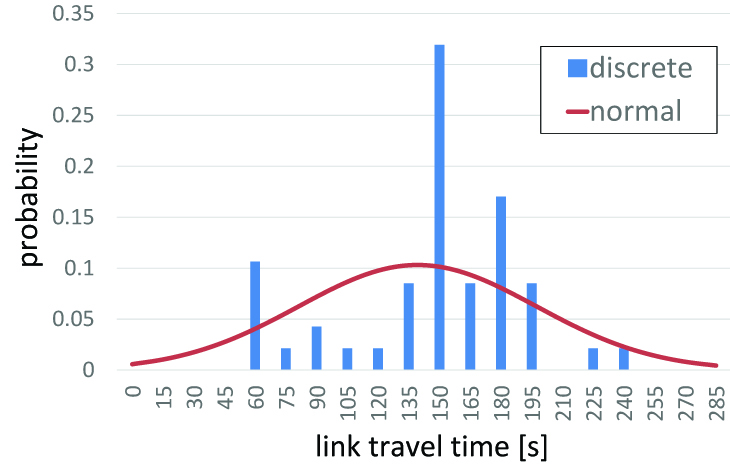
\includegraphics[width = 0.6\columnwidth]{figures/ltt_0900.jpg}
    }
    \subfigure[12:00pm]{
        \label{fig:1200}
        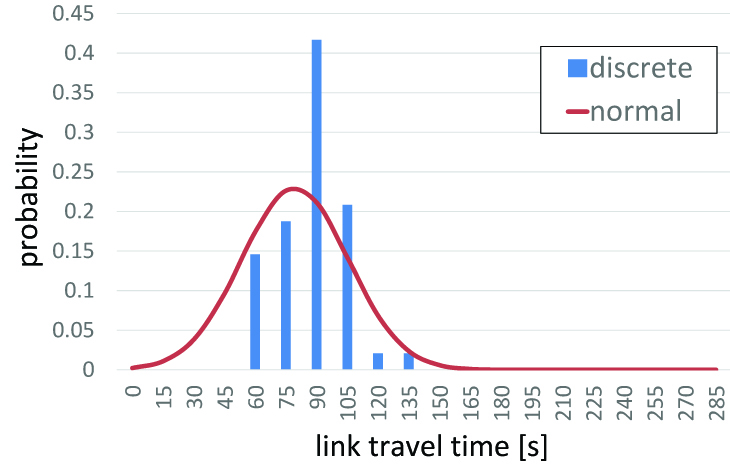
\includegraphics[width = 0.6\columnwidth]{figures/ltt_1200.jpg}
    }
    \subfigure[6:00pm]{
        \label{fig:1800}
        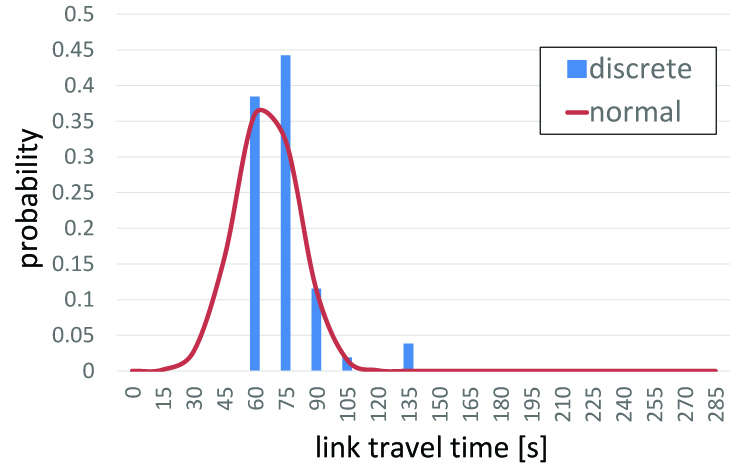
\includegraphics[width = 0.6\columnwidth]{figures/ltt_1800.jpg}
    }
    \caption{Historical model for a street segment for different times of a
    Monday}\label{fig:ltt}
\end{figure*}

In the remainder of this section, we will discuss our techniques to generate probabilistic link travel-times.

\subsection{Prediction through Historical Data}
\label{subsec:historical}
To obtain a \textit{pdf} representing $c_{ij}^{t_s}$ for a start time $(t_s \geq t_q)$ a simple approach is to use the available historical data. We define the set of historical data as $H = \{h | h < t_q\}$. Let us note that the link travel time $c_{ij}^h$ where $ h < t_q$ is not a random variable but a certain value which is known. In order to predict the travel time for time $t_s \geq t_q$ more accurately, we only consider a subset of historical data, $H^{t_s} \subset H$, with similar characteristics to time $t_s$. For example, if we want to predict the behaviour of edge $(i,j)$ at 9:00am for the next Tuesday, an adequate set $H^{t_s}$ might consist of data points $h$, where $h$ is 9:00am on a Tuesday in the last year. The travel time $c_{i,j}^h$ corresponding to last Friday 10:00pm might on the other hand, not be valuable in the prediction.

How to choose a set $H^{t_s}$ highly depends on the characteristics of the underlying traffic network. We use the results in \cite{Pan12} for choosing the appropriate $H^{t_s}$ for each start time. For a specific \textit{time of day} during a weekday, $H^{t_s}$ consists of data points corresponding to the same \textit{time of day} during \textbf{\textit{any}} weekday. For example, if the start time is 9:00am on this Tuesday, $H^{t_s}$ will consist of data points at 9:00am during Mondays, Tuesdays, Wednesdays, Thursdays and Fridays. The assumption is that traffic patters during weekdays are similar. More details can be found in \cite{Pan12}.

For continuous representation of the link travel time, we assume normal distribution with the following parameters
\begin{gather}
	\mu_{ij}^{t_s} = \frac{1}{|H^{t_s}|}\sum_{h\in H^{t_s}} c_{i,j}^h\\ 
	(\sigma_{ij}^{t_s})^2 = \frac{1}{|H^{t_s}|}\sum_{h\in H^{t_s}} (c_{ij}^h-\mu_{ij}^{t_s})^2\\
	\rho_{ij-kl} = \frac{\sum_{h\in H^{t_s}} (c_{ij}^h - \mu_{ij}) (c_{kl}^h -
	\mu_{kl})}{(|H^{t_s}|-1) \sigma_{ij} \sigma_{kl}}
\end{gather}

where $\rho$ is the Pearson correlation coefficient \cite{Soper17}

For the case of discrete representation through a \textit{pmf} we set

\begin{gather}
  F_{ij}^{t_s}(b) = \frac{1}{|H^{t_s}|}\sum_{h\in H^{t_s}} I(\lceil c_{ij}^h \rceil^\phi= b)
\end{gather}

where $\lceil x \rceil^\phi$ rounds $x$ up to the next multiple of $\phi$ and $I(c_{ij}^h = b)$ is an indicator variable which is 1 if $c_{ij}^h = b$ and 0 otherwise. The \textit{pmf} of each edge is thus given by a histogram assigning for each possible travel time of the edge a probability corresponding to its proportional occurrence in the historical data. 

\cref{fig:ltt} shows the discrete and continuous models of a typical inbound street segment of the network with a length of 1 mile for different times of the day. Based on the observation of historic patterns, in the morning a lot of traffic passes through this link. More traffic, intuitively, implies a higher probability of accidents which explains the rather large variation in the link travel time. At noon the traffic is reduced and in the evening the link travel time has the least amount of traffic, yielding the fastest travel time and in this case also the smallest variance. The figure also shows that the use of a normal distribution might not always adequately represent the link travel time.

We end this subsection with a note on \textit{query time} and \textit{prediction time}. When only historic data is used for prediction, the concept of prediction time becomes irrelevant. This means that if we are predicting for start time set to 9:00am today and we only use historic data, whether the query time is 7:00am or 8:00am does not make any difference since we only use $H^{t_s}$ corresponding to the start time to build the model. Prediction time and query time become important once we take the \textit{current situation} into account when building the prediction model which we will discuss in the following. 

\subsection{Historical Data and Current Situation}
The technique discussed in \cref{subsec:historical} provides link travel time distributions only based on historical data. These estimations may be a good choice if the start time $t_s$, for which the link travel time has to be predicted, is reasonably far (e.g., more than several hours) in the future. However, it may not be sufficient to capture current (and near future) traffic conditions with high confidence. For example, if we want to predict the travel time for 5 minutes later, the current situation of the road network might be more relevant than the historic data. Therefore, we present two estimation methods, incorporating both, the historical as well as the current link travel times of edges.

\subsubsection{Prediction through Linear Interpolation}
\label{subsec:LI}
The intuition of this approach is that 
\begin{itemize}
  \item for a start time $t_s$ which is far in the future, the historical prediction (\cref{subsec:historical}) is expected to yield a good prediction performance and
\item for the start time $t_s = t_q$, the current situation yields the best "prediction".
\end{itemize}

Thus, for a start time $t_s$ which is in the relatively near future, we argue that both, the historical as well as the current situation should influence the prediction. The closer the time $t_s$ is to $t_q$ (smaller prediction time) the more weight the current situation should have and vice versa. As the prediction time increases, we eventually get to a point where the current situation should loose it's influence. Towards this end we define a threshold parameter $\tau$, which defines the time-horizon in which the current situation has an influence on the prediction. Using a small time horizon $\tau$ is basically valuing the historic data, whereas setting $\tau$ to a larger value puts more weight on the current situation. We also define $\theta \in [0,1]$ as the relative importance of the current situation in the estimation. $\theta$ depends on the prediction time and is computed as:
\begin{equation}
\theta = min \{\frac{t_p}{\tau}, 1 \}
\end{equation}
where, as explained earlier, $t_p$ is the prediction time.

For continuous representation of link travel times, we estimate the parameters of the normal distribution as:

\begin{gather}
	\mu_{ij}^{t_s} = \left(\theta\cdot\frac{1}{|H^{t_s}|}\sum_{h\in H^{t_s}} c_{i,j}^h \right)
	+ \left(1-\theta\right)\cdot c_{i,j}^{t_q}\\
	(\sigma_{ij}^{t_s})^2 = \theta^2 \cdot \frac{1}{|H^{t_s}|}\sum_{h\in H^{t_s}}
	(c_{ij}^h-\mu_{ij}^{t_s})^2
\end{gather}

In particular, we perform a linear interpolation between the current link travel time, and the summarized historical link travel time in order to find the link travel time to be estimated. \cref{fig:interpolation} illustrates this concept, where  $\theta = 0.5$ and thus the expected value of the prediction is the average of the current situation and the predicted value by the historical approach. Accordingly, the standard deviation of the historical prediction is cut by half.

\begin{figure}[h]
    \centering
    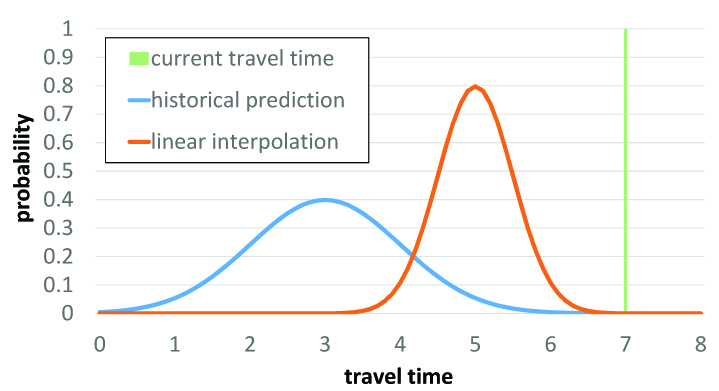
\includegraphics[width=0.80\columnwidth]{figures/tt_interpolation.jpg}
    \caption{Linear interpolation of ltt}
    \label{fig:interpolation}
\end{figure}

In the case of discrete link travel times, we adapt the same concept and obtain the following parameters.

\begin{gather}
F_{ij}^{t_s}(b) = \frac{1}{|H^{t_s}|}\sum_{h\in H^{t_s}} I(\lceil\theta \cdot 
c_{ij}^h + (1-\theta)\cdot c_{i,j}^{t_q}\rceil^\phi = b)
\end{gather}

where $\lceil x \rceil^\phi$ rounds $x$ up to the next multiple of $\phi$ and $I()$ is the indicator function.

\subsubsection{Prediction through Similar Historical Data}
\label{subsec:SH}
The third and final approach we propose is based on the idea that the current situation is a crucial indicator of how the travel time of a link will develop in the future. In this approach we use the current situation to further restricts the set $H^{t_s}$. Specifically we only include times $h \in H^{t_s}$, for which link $(i, j)$ had a travel time similar to the current situation at time $h-(t_p)$. In this context, we define similarity by a percentage threshold $\lambda$, which represents the deviation from the current travel time. To illustrate this idea, we provide an example. Assume we are predicting the travel time for link $l$ where $t_q=$ 7:00am and $t_s=$ 8:00am. We only consider the data points at 8:00am from days where the traffic at 7:00am was similar to today. For example, if the current travel time over link $l$, is 5 minutes and $\lambda = 0.2$, we only consider days where the travel time over link $l$ is somewhere between 4 minutes and 6 minutes.

We can formally define the further restricted set $H_{i,j}^{t_s}$ as:

\begin{equation}
H_{i,j}^{t_s} = \{h|h \in H^{t_s} \wedge \left| \frac{c_{i,j}^{t_q} - c_{i,j}^{h-t_p}}{c_{i,j}^{t_q}} \right| \leq \lambda \}  
\end{equation}

The value of $\lambda$ affects the prediction result. Setting $\lambda$ too small might result in not enough sample points. This can cause problems like over fitting the model. On the other hand setting $\lambda$ too large yields the historical prediction approach. In \cref{sec:experiments} we test with different values of $\lambda$ to find the optimal value for this parameter. 


